%! TEX root = gambar_alat.tex
% the main TeX file which is intended to compile, :VimtexReload after adjustment
   % this file should be included in the main file
% :h vimtex-tex-root
\documentclass[../menggambarteknik.tex]{subfiles}
%ensure the class of docs

\begin{document}


\section{Gambar Mur Baut}%
\label{sec:gambar_mur_baut}

\subsection{Tujuan}%
\label{sub:tujuan}

Setelah mempelajari bahan dalam bab ini, seharusnya Anda dapat:
\begin{itemize}
	\item Menjelaskan perbedaan gambar ulir luar (baut) dan ulir dalam (mur).
	\item Menggambar ulir luar dan ulir dalam.
	\item Menghitung dimensi mur-baut.
	\item Mendesain gambar mur-baut.
\end{itemize}

\subsection{Ulir Luar dan Ulir Dalam}%
\label{sub:ulir_luar_dan_ulir_dalam}

Dalam gambar teknik mesin hampir setiap saat selalu ada gambar ulir. Untuk itu juru gambar dan teknisi yang ada di industri harus mempunyai pengetahuan yang cukup mengenai tipe dan penggunaan ulir serta metode yang tepat untuk menggambarkannya, karena seringnya muncul ulir sekrup serta alat pengencang itu dalam konstruksi dan dalam mesin.

Untuk menggambar ulir yang sederhana diameter luar ulir digambar dengan garis tebal dan diameter dalamnya dengan garis tipis untuk gambar ulir luar (batangnya), sedangkan untuk ulir dalam (lubangnya) adalah sebaliknya. Pada ulir luar untuk pandangan depannya, diameter dalam ulir digambar ¾ lingkaran, sedangkan ¼ lingkaran bagian dikosongkan menggunakan garis tipis, penempatannya di sebelah kiri bawah. Untuk ulir dalam, pandangan depan diameter luar ulir digambar ¾ lingkaran, sedangkan ¼ lingkaran bagian luar dikosongkan, garisnya tipis, penempatannya disebelah kiri atas. Gambar~\ref{fig:gbr_ulir} memperlihatkan perbedaan penggambaran untuk ulir luar dan ulir dalam.

\begin{figure}
	\begin{center}
		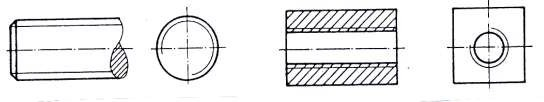
\includegraphics[width=.82\textwidth]{../figures/gbr_ulir.jpg}
		% filename may not contain space but _
	\end{center}
	\caption{Penggambaran Ulir Luar dan dalam}
	\label{fig:gbr_ulir}
\end{figure}

Ada dua cara untuk menggambar ujung baut, yaitu model lengkungan dan kerucut (Champer). Untuk ujung melengkung, jari-jarinya sama dengan diameter luar baut, sedangkan untuk model kerucut dichamper 450 (lihat gambar~\ref{fig:ujung_baut}).

\begin{figure}
	\begin{center}
		
\includegraphics[width=.72\textwidth]{ujung_baut}
		% filename may not contain space but _
	\end{center}
	\caption{Bentuk Ujung Baut}
	\label{fig:ujung_baut}
\end{figure}

\subsection{Gambar Pasangan Mur-Baut}%
\label{sub:gambar_pasangan_mur-baut}

Penggambaran mur-baut harus dilakukan dengan jelas, dengan demikian orang yang membaca gambar tahu bentuk sebenarnya dari mur-baut tersebut. Untuk menjelaskan bentuk ulir mur-baut hanya dengan menggunakan pandangan muka sebenarnya sudah cukup. Tetapi dalam hal-hal tertentu perlu untuk menggambarkannya dalam tiga pandangan yaitu pandangan muka, atas dan samping kanan, jika kita perlu mengetahui ukuran kepala tetap, tangkai dan kepala bautnya.
Sebagai pengikat yang berbentuk ulir, baut dan mur banyak digunakan dalam kontruksi permesinan. Bagian-bagian dari baut dan mur terdiri dari baut, kepala tetap baut dan mur. Bentuk kepala tetap baut dan mur adalah biasanya segi empat atau segi enam. Pada umumnya baut dan mur tidak digambar pada detail (bagian), tetapi dalam gambar susunan biasanya digambar sesuai dengan standar yang ada menurut perbandingan diameter luar yang aturannya seperti pada gambar~\ref{fig:gbr_baut} di bawah ini.

\begin{figure}
	\begin{center}
		
\includegraphics[width=.82\textwidth]{gbr_baut}
		% filename may not contain space but _
	\end{center}
	\caption{Cara Menggambar baut, kepalla tetap dan mur}
	\label{fig:gbr_baut}
\end{figure}

\section{Gambar Roda Gigi}%
\label{sec:Gambar Roda Gigi}

\subsection{Tujuan}%
\label{sub:tujuan}

Setelah mempelajari bahan dalam bab ini, seharusnya Anda dapat:

\begin{itemize}
	\item Menunjukkan cara menggambar roda gigi.
	\item Mengidentifikasi macam-macam roda gigi.
	\item Membaca dan menggambar macam-macam roda gigi.
\end{itemize}

\subsection{Cara Menggambar Roda Gigi}%
\label{sub:cara_menggambar_roda_gigi}


Roda gigi adalah merupakan bagian yang penting pada mesin-mesin penggerak, dimana roda gigi ini akan menghubungkan dan meneruskan gerak dan gaya transmisi. Adanya pasangan roda gigi ini memungkinkan untuk mempercepat atau memperlambat kecepatan putar dalam rangkaian transmisi yang ada, sehingga apabila diinginkan putaran yang lambat, maka roda gigi yang digerakan bisa diperbesar demikian pula sebaliknya.

Sebagai elemen bentuk yang mengulang roda gigi dapat digambarkan secara konvensional dalam cara yang disederhanakan sebagai roda pejal dengan lingkaran jaraknya digambar dengan garis sumbu tipis. Untuk itu suatu gambar rangkaian roda gigi paling tidak harus mencakup hal-hal sebagai berikut:

\begin{itemize}
	\item Pandangan depan roda gigi adalah pandangan yang memperlihatkan sumbu lubang porosnya. Garis kepala atau lingkaran kepala digambar dengan garis tebal, dan garis jarak antara atau lingkaran jarak dengan garis sumbu tipis.
	\item Garis kaki atau lingkaran kaki digambar dengan garis tipis, tetapi dapat dihilangkan juga. Gambar pandangan depan yang dipotong harus memperlihatkan lingkaran kaki dengan garis tebal.
	\item Arah gigi dari roda gigi dengan gigi miring bila perlu diperlihatkan dapat digambar dengan tiga garis tipis, yang menunjukkan arah dan bentuk giginya.
\end{itemize}

Selain pandangan yang tepat dengan menggunakan garis yang sesuai, dalam  menggambar  roda  gigi  dianjurkan  untuk  memberikan  ukuran  pada pandangan-pandangan gambar yang dibuat. Ukuran-ukuran ini akan dapat menjadi keterangan yang diperlukan dalam pembuatannya. Apabila diperlukan keterangan yang lain, maka dapat diletakkan dalam tabel data gigi yang ada pada etiket gambar.
Gambar~\ref{fig:gbr_roda_gigi}. Memperlihatkan contoh cara menggambar roda gigi.

\begin{figure}
	\begin{center}
		
\includegraphics[width=.82\textwidth]{gbr_roda_gigi}
		% filename may not contain space but _
	\end{center}
	\caption{Contoh Cara menggambar roda gigi}
	\label{fig:gbr_roda_gigi}
\end{figure}

\subsection{Macam-Macam Pasangan Roda Gigi}%
\label{sub:macam-macam_pasangan_roda_gigi}

Untuk menyusun gambar rangkaian roda gigi, aturan-aturan yang dipergunakan pada roda gigi tunggal tetap dapat dipergunakan. Gambar pandangan depan yang dipotong salah satu giginya tertutup oleh gigi yang lain dan digambar dengan garis gores, sedangkan yang satu lagi digambar dengan garis tebal. Sedangkan bila pandangan depan tidak dipotong, masing-masing kepala gigi digambar dengan garis tebal. Ketika menggambar rangkaian roda gigi, seorang juru gambar atau teknisi perlu untuk mengetahui bentuk-bentuk roda gigi. Adapun macam-macam rangkaian pasangan roda gigi secara ringkas dapat dibedakan menjadi lima macam, yaitu: pasangan roda gigi lurus, pasangan roda gigi cacing, pasangan roda gigi kerucut, pasangan roda gigi dengan batang gigi, dan pasangan roda gigi dalam (lihat gambar~\ref{fig:macam_roda_gigi}).


\begin{figure}
	\begin{center}
		
\includegraphics[width=.82\textwidth]{macam_roda_gigi}
		% filename may not contain space but _
	\end{center}
	\caption{Macam-macam pasangan roda gigi}
	\label{fig:macam_roda_gigi}
\end{figure}












\bibliographystyle{apalike}
\bibliography{../filename.bib} % required for citecompletion, not work in mainfile
\end{document}

